\documentclass{article}

\usepackage{cmlgc}
\usepackage{enumitem}
\usepackage{graphicx}
\usepackage{geometry}
\geometry{
    a4paper
}
\usepackage{hyperref}
\hypersetup{
    colorlinks=true,
    linkcolor=blue,
    urlcolor=blue
}
\usepackage{tabto}

\pagestyle{empty}
 
\begin{document}

\newgeometry{
    top=10mm,
    bottom=10mm,
    left=10mm,
    right=10mm
}

\begin{minipage}{1\textwidth}
    \begin{minipage}{.5\textwidth}
        \vspace{.2cm}
        {\huge \textbf{Vadim \textsc{Bertrand}}}\\[.3 cm]
        \url{https://github.com/vadmbertr/}
    \end{minipage}
    \begin{minipage}{.44\textwidth}
    \begin{flushright}
        \begin{minipage}{.74\textwidth}
        \begin{flushright}
            \href{tel:33614623218}{+33 6 14 62 32 18} \\[.1 cm]
            \href{mailto:vadim.bertrand@gmail.com}{vadim.bertrand@gmail.com} \\[.1 cm]
            Grenoble area \\[.1 cm]
            France
        \end{flushright}
        \end{minipage}
        \begin{minipage}{.24\textwidth}
        \begin{flushright}
            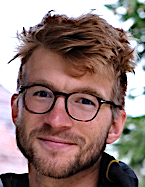
\includegraphics[width=1\textwidth]{picture.png}
        \end{flushright}
        \end{minipage}
    \end{flushright}
    \end{minipage}
\end{minipage}
\\[.1 cm]

\begin{center}
    \large{\textbf{2\textsuperscript{nd} year PhD student in Oceanography - Master's Degree in Statistics - Software Engineer}}
\end{center}

\section*{\textsc{Education}}
\begin{itemize}
    \item[] 2024— \tabto{2cm} \textbf{PhD}, Institut des Géosciences de l'Environnement - Team \textbf{MEOM} \\[.1 cm]
    \tabto{2cm} \textit{Stochastic Modelling of Drifting Object Trajectories at the Ocean Surface using Machine Learning} \\[.1 cm]
    \tabto{2cm} Supervised by Julien Le Sommer (CNRS Researcher), Emmanuel Cosme (UGA Professor) and \tabto{2cm} Adeline Leclercq Samson (UGA Professor)
    \vspace{-.1 cm}
    \begin{itemize}[left=2cm]
        \item[$\rightarrow$] Implementing the \texttt{Python} package \href{https://github.com/vadmbertr/pastax}{\texttt{pastax}}
    \end{itemize}
    \item[] 2023 \tabto{2cm} \textbf{Master’s Degree in Statistics and Data Science}, Université Grenoble Alpes - IM\textsuperscript{2}AG \\[.15 cm]
    \tabto{2cm} \textit{Graduated with High Honors} \\[.1 cm]
    \tabto{2cm} Bayesian statistics, Computational statistics, Spatial statistics, Operations research and optimization, \tabto{2cm} Non-parametric and functional estimation, Supervised and unsupervised learning
    \item[] 2014 \tabto{2cm} \textbf{Engineering Degree}, Grenoble INP - Phelma / Ensimag \\[.1 cm]
    \tabto{2cm} Signal processing, Algorithms and programming, Graph theory, Information theory
\end{itemize}

\section*{\textsc{Academic and Professional Experience}}
\begin{itemize}
    \item[] 2024—2025 \tabto{2cm} \textbf{Summer School}, \href{https://oceantrainingcourse2025.esa.int/}{Ocean Training Course 2025} – Organized by the European Space Agency \\[.1 cm]
    \tabto{2cm} \textit{Advanced Training Course on Ocean Synergy Remote Sensing} focusing on the joint use of satellite and \tabto{2cm} in-situ instruments to observe oceanic and atmospheric processes \\[.1 cm]
    \tabto{2cm} \underline{Shore-based} component of 14 training sessions on different Earth Observation satellite measurements \\[.1 cm]
    \tabto{2cm} \underline{Ship-based} component of 6 weeks from Tromsø (Norway) to Nice (France) aboard the \href{https://lehmkuhl.no/en/}{Statsraad Lehmkuhl}
    \vspace{-.4 cm}
    \begin{itemize}[left=2cm]
        \item[$\rightarrow$] Designed and assembled low-cost surface drifters deployed during the campaign, more details \href{https://github.com/vadmbertr/otc25-cannelloni}{here}
        \item[$\rightarrow$] Organized a drifter position prediction challenge taking place during the shipboard training, see \href{https://vadmbertr.github.io/otc25-virtual-drift/}{here}
    \end{itemize}

    \item[] 2023 \tabto{2cm} \textbf{Research Engineer}, Institut des Géosciences de l'Environnement – Team \textbf{MEOM} \\[.1 cm]
    \tabto{2cm} \textit{Variational cyclogeostrophic inversion for estimating ocean surface currents} \\[.1 cm]
    \tabto{2cm} Supervised by Emmanuel Cosme (UGA Full Professor) and Julien Le Sommer (CNRS Researcher)
    \vspace{-.1 cm}
    \begin{itemize}[left=2cm]
        \item[$\rightarrow$] Implemented the \texttt{Python} package \href{https://github.com/meom-group/jaxparrow}{\texttt{jaxparrow}}, leveraging \texttt{JAX}. \href{https://doi.org/10.5281/zenodo.14871648}{10.5281/zenodo.14871648}
    \end{itemize}
    
    \item[] 2023 \tabto{2cm} \textbf{Research Internship}, TIMC – Team \textbf{M}odels and \textbf{A}lgorithms for \textbf{Ge}nomics \\[.1 cm]
    \tabto{2cm} \textit{Exploration of joint deconvolution algorithms for omic data} (\href{https://vadmbertr.github.io/material/reports/M2_Internship_report__Exploration_of_joint_deconvolution_algorithms_for_omic_data.pdf}{report}, \href{https://vadmbertr.github.io/material/posters/poster_jobim_ismb.pdf}{poster}) \\[.1 cm]
    \tabto{2cm} Supervised by Magali Richard (CNRS Researcher)
    
    \item[] 2022—2023 \tabto{2cm} \textbf{Mentored Master's Project}, Université Grenoble Alpes - IM\textsuperscript{2}AG \\[.1 cm]
    \tabto{2cm} \textit{Effect of anthropogenic noise on narwhals behavior} (as part of \href{https://doi.org/10.1126/sciadv.ade0440}{this larger study}) \\[.1 cm]
    \tabto{2cm} Supervised by Adeline Leclercq Samson (UGA Full Professor)
    
    \item[] 2022 \tabto{2cm} \textbf{Research Internship}, Laboratoire Jean Kuntzmann - Team \textbf{D}onnées, \textbf{A}pprentissage et \textbf{O}ptimisation \\[.1 cm]
    \tabto{2cm} \textit{Deep generative learning for next-generation drugs} (\href{https://vadmbertr.github.io/material/reports/Internship_report___Deep_generative_learning_for_next_generation_drugs.pdf}{report}) \\[.1 cm]
    \tabto{2cm} Supervised by Sergei Grudinin (CNRS Researcher)
    
    \item[] 2016—2021 \tabto{2cm} \textbf{Software Engineer}, Inria / GIPSA-lab - Team \textbf{D}ynamics \textbf{an}d \textbf{C}ontrol of N\textbf{e}tworks\\[.1 cm]
    \tabto{2cm} Supervised by Carlos Canudas-de-Wit (CNRS Researcher)
    \vspace{-.1cm}
    \begin{itemize}[left=2cm]
        \item[$\rightarrow$] Developed the web-application \href{https://gtlville.inrialpes.fr/}{GTL-VILLE}, collecting, estimating and predicting road traffic indicators in real time in the Grenoble Metropolis (\href{https://hal.science/hal-03694936}{subsequent publication})
    \end{itemize}
\end{itemize}

\section*{\textsc{Teaching}}
\begin{itemize}
    \item[] 2024 \tabto{2cm} \textbf{Computing and Data Analysis Project (Supervision of 2 students)}, Université Grenoble Alpes - \tabto{2cm} Master in Earth, planetary and environmental sciences
    \item[] 2024 \tabto{2cm} \textbf{Statistics (Practical Session)}, Université Grenoble Alpes - Bachelor in Biochemistry
\end{itemize}

\section*{\textsc{Internship Supervision}}
\begin{itemize}
    \item[] 2024 \tabto{2cm} \textbf{Léo Boux de Casson (Bachelor, École Normale Supérieure de Lyon)}, with Julien Le Sommer \\[.1 cm]
    \tabto{2cm} \textit{Eulerian comparison of lagrangian drifter velocities and reconstructed sea surface currents within the \tabto{2cm} SWOT swath in the Mediterranean sea}
    \item[] 2017 \tabto{2cm} \textbf{Baptiste Gouin (Master, Université Paris Sud)}, with Giacomo Casadei \\[.1 cm]
    \tabto{2cm} \textit{Aggregation and travel time calculation over large scale traffic networks}
\end{itemize}

\section*{\textsc{Scientific Activities}}
\begin{itemize}
    \item[] 2025 \tabto{2cm} \textbf{Journal Article} \textit{in preparation} - V. Bertrand, J. Le Sommer, V. Zaia De Almeida, A. \tabto{2cm} Samson, E. Cosme, \textit{A Robust Variational Framework for Cyclogeostrophic Ocean Surface Current Retrieval.}

    \item[] 2024 \tabto{2cm} \textbf{Journal Article} \textit{under review at Genomic Biology} - E. Amblard, V. Bertrand, L. Martin Pena, S. Karkar, \tabto{2cm} F. Chuffart, M. Ayadi, A. Baurès, L. Armenoult, Y. Kermezli, J. Cros, Y. Blum, M. Richard, \textit{A robust \tabto{2cm} workflow to benchmark deconvolution of multi-omic data.} \href{https://doi.org/10.1101/2024.11.08.622633}{10.1101/2024.11.08.622633}

    \item[] 2025 \tabto{2cm} \textbf{Hackathon} - Attendee in the \href{https://github.com/Diff4Earth/ige-jaxathon-2025}{JAXATHON} organized at IGE, Grenoble, France. \\[.1 cm]
        \tabto{2cm} Gave an informal presentation of the JAX ecosystem. \href{https://vadmbertr.github.io/material/presentations/2025-03-jaxathon.pdf}{PDF}

    \item[] 2024 \tabto{2cm} \textbf{Poster Presentation} - \textit{Stochastic and differentiable simulators of drifting objects trajectories}, EDITO \tabto{2cm} WP2 Workshop, Grenoble, France. \href{https://vadmbertr.github.io/material/posters/2024-10_EDITO_Bertrand.pdf}{PDF}
    
    \item[] 2024 \tabto{2cm} \textbf{Oral Presentation} - \textit{Cyclogeostrophic inversion for estimating Sea Surface Currents from SWOT \tabto{2cm} altimeter data}, 30YPRA-OSTST, Montpellier, France. \href{https://vadmbertr.github.io/material/presentations/2.4-5-Bertrand.pdf}{PDF}
    
    \item[] 2024 \tabto{2cm} \textbf{Poster Presentation} - \textit{Cyclogeostrophic inversion for estimating Sea Surface Currents}, EGU, Vienna, \tabto{2cm} Austria. \href{https://doi.org/10.5194/egusphere-egu24-17489}{10.5194/egusphere-egu24-17489}
    
    \item[] 2023 \tabto{2cm} \textbf{Poster Presentation} - \textit{Scoring and ranking strategies to benchmark cell type deconvolution pipelines}, \tabto{2cm} JOBIM and ISMB, Nice and Lyon, France. \href{https://vadmbertr.github.io/material/posters/poster_jobim_ismb.pdf}{PDF}
    
    \item[] 2018 \tabto{2cm} \textbf{Journal Article} - G. Casadei, V. Bertrand, B. Gouin, C. Canudas-de-Wit, \textit{Aggregation and travel time \tabto{2cm} calculation over large scale traffic networks: An empiric study on the Grenoble City}. Transportation \tabto{2cm} Research Part C: Emerging Technologies, 2018. \href{https://doi.org/10.1016/j.trc.2018.07.033}{10.1016/j.trc.2018.07.033}
\end{itemize}

\section*{\textsc{Open Source Contributions}}
\begin{itemize}
    \item[] \textbf{Personal Projects}, developper and maintainer of:
        \begin{itemize}[leftmargin=2cm]
            \item[] \href{https://github.com/vadmbertr/pastax}{\texttt{pastax}} \textit{Parameterizable Auto-differentiable Simulators of ocean Trajectories in jAX}
            \item[] \href{https://github.com/meom-group/jaxparrow}{\texttt{jaxparrow}} \textit{A package for computing the inversion of the cyclogeostrophic balance based on a variational formulation approach}. \href{https://doi.org/10.5281/zenodo.14871648}{10.5281/zenodo.14871648}
        \end{itemize}
    \item[] \textbf{Community Projects}, contributor to:
        \begin{itemize}[leftmargin=2cm]
            \item[] \href{https://github.com/Cloud-Drift/clouddrift}{\texttt{clouddrift}} \textit{Accelerates the use of Lagrangian data for atmospheric, oceanic, and climate sciences}
            \item[] \href{https://github.com/patrick-kidger/quax}{\texttt{quax}} \textit{Multiple dispatch over abstract array types in JAX}
            \item[] \href{https://github.com/meom-group/widetrax}{\texttt{widetrax}} \textit{Toolbox for manipulating wide-swath altimetry ocean data}
        \end{itemize}
\end{itemize}

\section*{\textsc{Miscellaneous}}
\begin{itemize}
    \item[] \textbf{Living languages} \\[.1 cm] 
        \tabto{2cm} English: fluent, Spanish: notions
    \item[] \textbf{Programming languages} \\[.1 cm] 
        \tabto{2cm} Python (JAX, PyTorch, NumPy, Xarray, etc...), Julia, R ; Git ; Shell scripting
    \item[] \textbf{Hobbies} \\[.1 cm] 
        \tabto{2cm} Rugby (2 years in sports study) and now Touch rugby (\href{https://youtu.be/yE_VXFf4pCk?si=aiIs_IFJW4eTuIwQ}{what is this?}), Running, Ski touring, Diving
\end{itemize}

\end{document}
